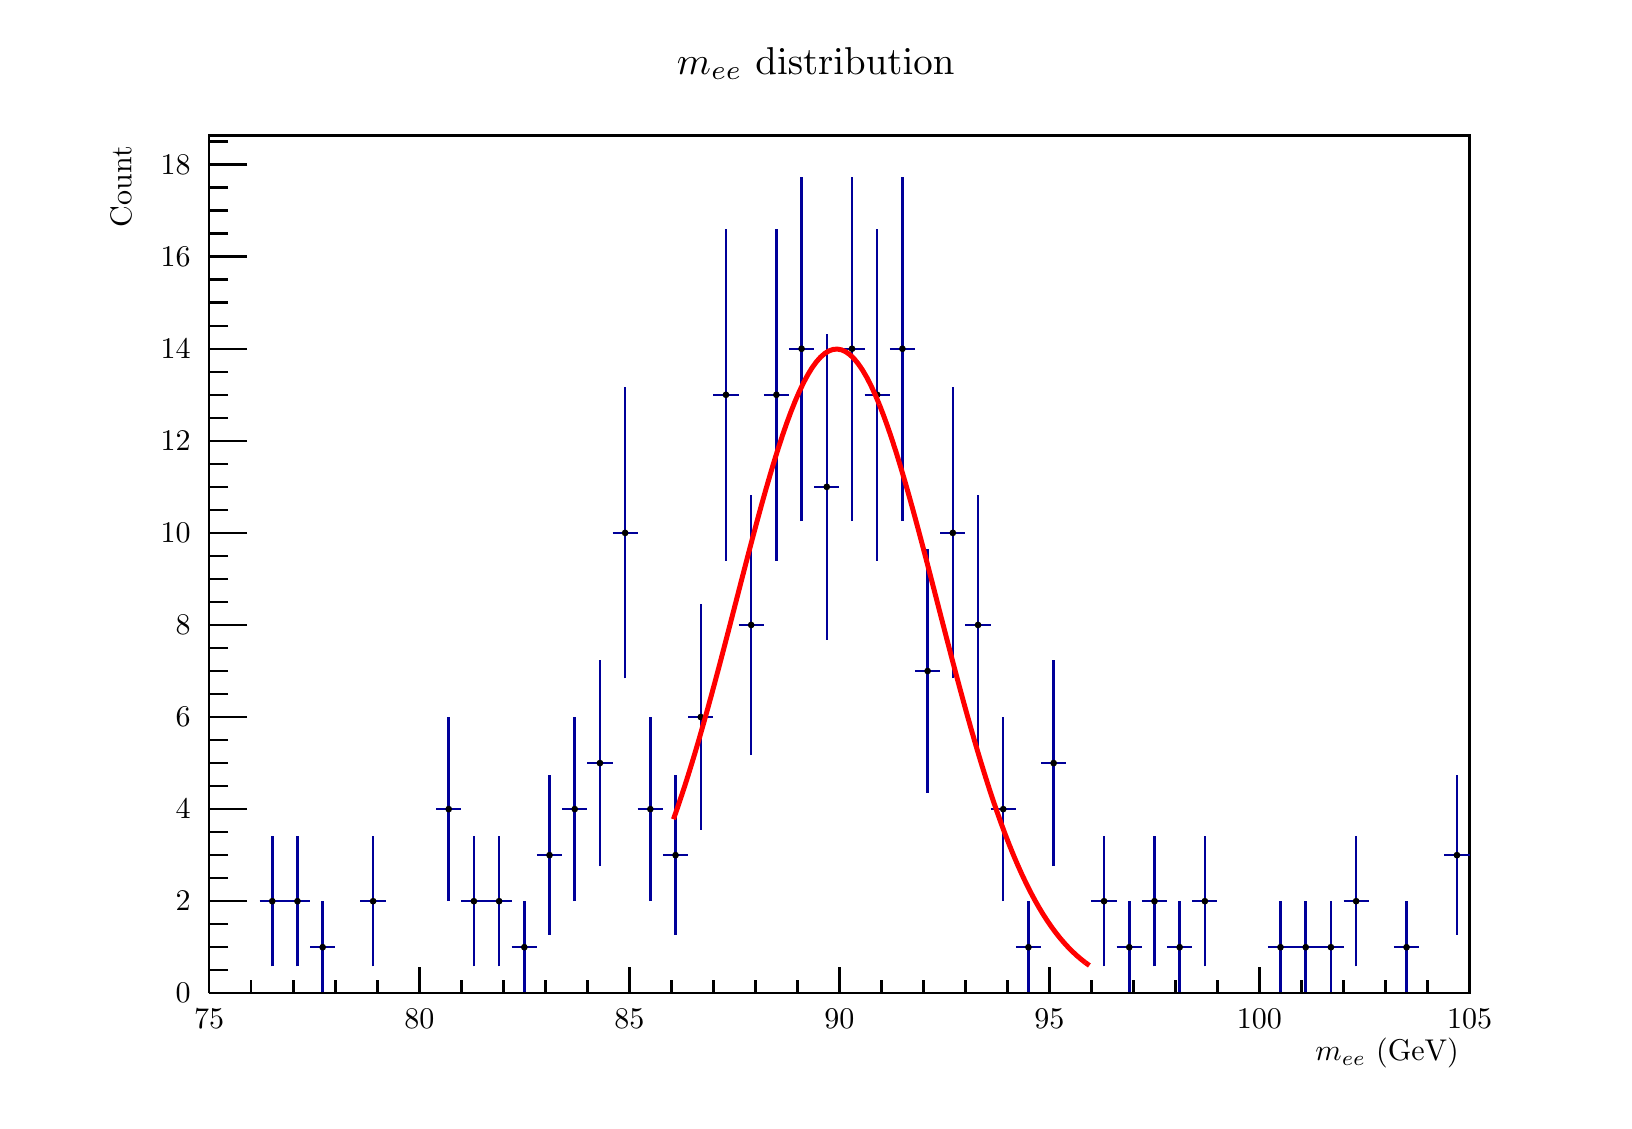
\begin{tikzpicture}
\pgfdeclareplotmark{cross} {
\pgfpathmoveto{\pgfpoint{-0.3\pgfplotmarksize}{\pgfplotmarksize}}
\pgfpathlineto{\pgfpoint{+0.3\pgfplotmarksize}{\pgfplotmarksize}}
\pgfpathlineto{\pgfpoint{+0.3\pgfplotmarksize}{0.3\pgfplotmarksize}}
\pgfpathlineto{\pgfpoint{+1\pgfplotmarksize}{0.3\pgfplotmarksize}}
\pgfpathlineto{\pgfpoint{+1\pgfplotmarksize}{-0.3\pgfplotmarksize}}
\pgfpathlineto{\pgfpoint{+0.3\pgfplotmarksize}{-0.3\pgfplotmarksize}}
\pgfpathlineto{\pgfpoint{+0.3\pgfplotmarksize}{-1.\pgfplotmarksize}}
\pgfpathlineto{\pgfpoint{-0.3\pgfplotmarksize}{-1.\pgfplotmarksize}}
\pgfpathlineto{\pgfpoint{-0.3\pgfplotmarksize}{-0.3\pgfplotmarksize}}
\pgfpathlineto{\pgfpoint{-1.\pgfplotmarksize}{-0.3\pgfplotmarksize}}
\pgfpathlineto{\pgfpoint{-1.\pgfplotmarksize}{0.3\pgfplotmarksize}}
\pgfpathlineto{\pgfpoint{-0.3\pgfplotmarksize}{0.3\pgfplotmarksize}}
\pgfpathclose
\pgfusepathqstroke
}
\pgfdeclareplotmark{cross*} {
\pgfpathmoveto{\pgfpoint{-0.3\pgfplotmarksize}{\pgfplotmarksize}}
\pgfpathlineto{\pgfpoint{+0.3\pgfplotmarksize}{\pgfplotmarksize}}
\pgfpathlineto{\pgfpoint{+0.3\pgfplotmarksize}{0.3\pgfplotmarksize}}
\pgfpathlineto{\pgfpoint{+1\pgfplotmarksize}{0.3\pgfplotmarksize}}
\pgfpathlineto{\pgfpoint{+1\pgfplotmarksize}{-0.3\pgfplotmarksize}}
\pgfpathlineto{\pgfpoint{+0.3\pgfplotmarksize}{-0.3\pgfplotmarksize}}
\pgfpathlineto{\pgfpoint{+0.3\pgfplotmarksize}{-1.\pgfplotmarksize}}
\pgfpathlineto{\pgfpoint{-0.3\pgfplotmarksize}{-1.\pgfplotmarksize}}
\pgfpathlineto{\pgfpoint{-0.3\pgfplotmarksize}{-0.3\pgfplotmarksize}}
\pgfpathlineto{\pgfpoint{-1.\pgfplotmarksize}{-0.3\pgfplotmarksize}}
\pgfpathlineto{\pgfpoint{-1.\pgfplotmarksize}{0.3\pgfplotmarksize}}
\pgfpathlineto{\pgfpoint{-0.3\pgfplotmarksize}{0.3\pgfplotmarksize}}
\pgfpathclose
\pgfusepathqfillstroke
}
\pgfdeclareplotmark{newstar} {
\pgfpathmoveto{\pgfqpoint{0pt}{\pgfplotmarksize}}
\pgfpathlineto{\pgfqpointpolar{44}{0.5\pgfplotmarksize}}
\pgfpathlineto{\pgfqpointpolar{18}{\pgfplotmarksize}}
\pgfpathlineto{\pgfqpointpolar{-20}{0.5\pgfplotmarksize}}
\pgfpathlineto{\pgfqpointpolar{-54}{\pgfplotmarksize}}
\pgfpathlineto{\pgfqpointpolar{-90}{0.5\pgfplotmarksize}}
\pgfpathlineto{\pgfqpointpolar{234}{\pgfplotmarksize}}
\pgfpathlineto{\pgfqpointpolar{198}{0.5\pgfplotmarksize}}
\pgfpathlineto{\pgfqpointpolar{162}{\pgfplotmarksize}}
\pgfpathlineto{\pgfqpointpolar{134}{0.5\pgfplotmarksize}}
\pgfpathclose
\pgfusepathqstroke
}
\pgfdeclareplotmark{newstar*} {
\pgfpathmoveto{\pgfqpoint{0pt}{\pgfplotmarksize}}
\pgfpathlineto{\pgfqpointpolar{44}{0.5\pgfplotmarksize}}
\pgfpathlineto{\pgfqpointpolar{18}{\pgfplotmarksize}}
\pgfpathlineto{\pgfqpointpolar{-20}{0.5\pgfplotmarksize}}
\pgfpathlineto{\pgfqpointpolar{-54}{\pgfplotmarksize}}
\pgfpathlineto{\pgfqpointpolar{-90}{0.5\pgfplotmarksize}}
\pgfpathlineto{\pgfqpointpolar{234}{\pgfplotmarksize}}
\pgfpathlineto{\pgfqpointpolar{198}{0.5\pgfplotmarksize}}
\pgfpathlineto{\pgfqpointpolar{162}{\pgfplotmarksize}}
\pgfpathlineto{\pgfqpointpolar{134}{0.5\pgfplotmarksize}}
\pgfpathclose
\pgfusepathqfillstroke
}
\definecolor{c}{rgb}{1,1,1};
\draw [color=c, fill=c] (0,0) rectangle (20,13.6207);
\draw [color=c, fill=c] (2.29885,1.36494) rectangle (18.3046,12.2557);
\definecolor{c}{rgb}{0,0,0};
\draw [c,line width=0.9] (2.29885,1.36494) -- (2.29885,12.2557) -- (18.3046,12.2557) -- (18.3046,1.36494) -- (2.29885,1.36494);
\definecolor{c}{rgb}{1,1,1};
\draw [color=c, fill=c] (2.29885,1.36494) rectangle (18.3046,12.2557);
\definecolor{c}{rgb}{0,0,0};
\draw [c,line width=0.9] (2.29885,1.36494) -- (2.29885,12.2557) -- (18.3046,12.2557) -- (18.3046,1.36494) -- (2.29885,1.36494);
\definecolor{c}{rgb}{0,0,0.6};
\draw [c,line width=0.9] (3.09914,1.70741) -- (3.09914,2.53419);
\draw [c,line width=0.9] (3.09914,2.53419) -- (3.09914,3.36097);
\draw [c,line width=0.9] (2.93908,2.53419) -- (3.09914,2.53419);
\draw [c,line width=0.9] (3.09914,2.53419) -- (3.2592,2.53419);
\definecolor{c}{rgb}{0,0,0};
\foreach \P in {(3.09914,2.53419)}{\draw[mark options={color=c,fill=c},mark size=2.402402pt,mark=*,mark size=1pt] plot coordinates {\P};}
\definecolor{c}{rgb}{0,0,0.6};
\draw [c,line width=0.9] (3.41925,1.70741) -- (3.41925,2.53419);
\draw [c,line width=0.9] (3.41925,2.53419) -- (3.41925,3.36097);
\draw [c,line width=0.9] (3.2592,2.53419) -- (3.41925,2.53419);
\draw [c,line width=0.9] (3.41925,2.53419) -- (3.57931,2.53419);
\definecolor{c}{rgb}{0,0,0};
\foreach \P in {(3.41925,2.53419)}{\draw[mark options={color=c,fill=c},mark size=2.402402pt,mark=*,mark size=1pt] plot coordinates {\P};}
\definecolor{c}{rgb}{0,0,0.6};
\draw [c,line width=0.9] (3.73937,1.36494) -- (3.73937,1.94957);
\draw [c,line width=0.9] (3.73937,1.94957) -- (3.73937,2.53419);
\draw [c,line width=0.9] (3.57931,1.94957) -- (3.73937,1.94957);
\draw [c,line width=0.9] (3.73937,1.94957) -- (3.89943,1.94957);
\definecolor{c}{rgb}{0,0,0};
\foreach \P in {(3.73937,1.94957)}{\draw[mark options={color=c,fill=c},mark size=2.402402pt,mark=*,mark size=1pt] plot coordinates {\P};}
\definecolor{c}{rgb}{0,0,0.6};
\draw [c,line width=0.9] (4.3796,1.70741) -- (4.3796,2.53419);
\draw [c,line width=0.9] (4.3796,2.53419) -- (4.3796,3.36097);
\draw [c,line width=0.9] (4.21954,2.53419) -- (4.3796,2.53419);
\draw [c,line width=0.9] (4.3796,2.53419) -- (4.53966,2.53419);
\definecolor{c}{rgb}{0,0,0};
\foreach \P in {(4.3796,2.53419)}{\draw[mark options={color=c,fill=c},mark size=2.402402pt,mark=*,mark size=1pt] plot coordinates {\P};}
\definecolor{c}{rgb}{0,0,0.6};
\draw [c,line width=0.9] (5.33994,2.53419) -- (5.33994,3.70344);
\draw [c,line width=0.9] (5.33994,3.70344) -- (5.33994,4.87268);
\draw [c,line width=0.9] (5.17988,3.70344) -- (5.33994,3.70344);
\draw [c,line width=0.9] (5.33994,3.70344) -- (5.5,3.70344);
\definecolor{c}{rgb}{0,0,0};
\foreach \P in {(5.33994,3.70344)}{\draw[mark options={color=c,fill=c},mark size=2.402402pt,mark=*,mark size=1pt] plot coordinates {\P};}
\definecolor{c}{rgb}{0,0,0.6};
\draw [c,line width=0.9] (5.66006,1.70741) -- (5.66006,2.53419);
\draw [c,line width=0.9] (5.66006,2.53419) -- (5.66006,3.36097);
\draw [c,line width=0.9] (5.5,2.53419) -- (5.66006,2.53419);
\draw [c,line width=0.9] (5.66006,2.53419) -- (5.82012,2.53419);
\definecolor{c}{rgb}{0,0,0};
\foreach \P in {(5.66006,2.53419)}{\draw[mark options={color=c,fill=c},mark size=2.402402pt,mark=*,mark size=1pt] plot coordinates {\P};}
\definecolor{c}{rgb}{0,0,0.6};
\draw [c,line width=0.9] (5.98017,1.70741) -- (5.98017,2.53419);
\draw [c,line width=0.9] (5.98017,2.53419) -- (5.98017,3.36097);
\draw [c,line width=0.9] (5.82012,2.53419) -- (5.98017,2.53419);
\draw [c,line width=0.9] (5.98017,2.53419) -- (6.14023,2.53419);
\definecolor{c}{rgb}{0,0,0};
\foreach \P in {(5.98017,2.53419)}{\draw[mark options={color=c,fill=c},mark size=2.402402pt,mark=*,mark size=1pt] plot coordinates {\P};}
\definecolor{c}{rgb}{0,0,0.6};
\draw [c,line width=0.9] (6.30029,1.36494) -- (6.30029,1.94957);
\draw [c,line width=0.9] (6.30029,1.94957) -- (6.30029,2.53419);
\draw [c,line width=0.9] (6.14023,1.94957) -- (6.30029,1.94957);
\draw [c,line width=0.9] (6.30029,1.94957) -- (6.46034,1.94957);
\definecolor{c}{rgb}{0,0,0};
\foreach \P in {(6.30029,1.94957)}{\draw[mark options={color=c,fill=c},mark size=2.402402pt,mark=*,mark size=1pt] plot coordinates {\P};}
\definecolor{c}{rgb}{0,0,0.6};
\draw [c,line width=0.9] (6.6204,2.10622) -- (6.6204,3.11881);
\draw [c,line width=0.9] (6.6204,3.11881) -- (6.6204,4.13141);
\draw [c,line width=0.9] (6.46034,3.11881) -- (6.6204,3.11881);
\draw [c,line width=0.9] (6.6204,3.11881) -- (6.78046,3.11881);
\definecolor{c}{rgb}{0,0,0};
\foreach \P in {(6.6204,3.11881)}{\draw[mark options={color=c,fill=c},mark size=2.402402pt,mark=*,mark size=1pt] plot coordinates {\P};}
\definecolor{c}{rgb}{0,0,0.6};
\draw [c,line width=0.9] (6.94052,2.53419) -- (6.94052,3.70344);
\draw [c,line width=0.9] (6.94052,3.70344) -- (6.94052,4.87268);
\draw [c,line width=0.9] (6.78046,3.70344) -- (6.94052,3.70344);
\draw [c,line width=0.9] (6.94052,3.70344) -- (7.10057,3.70344);
\definecolor{c}{rgb}{0,0,0};
\foreach \P in {(6.94052,3.70344)}{\draw[mark options={color=c,fill=c},mark size=2.402402pt,mark=*,mark size=1pt] plot coordinates {\P};}
\definecolor{c}{rgb}{0,0,0.6};
\draw [c,line width=0.9] (7.26063,2.9808) -- (7.26063,4.28806);
\draw [c,line width=0.9] (7.26063,4.28806) -- (7.26063,5.59532);
\draw [c,line width=0.9] (7.10057,4.28806) -- (7.26063,4.28806);
\draw [c,line width=0.9] (7.26063,4.28806) -- (7.42069,4.28806);
\definecolor{c}{rgb}{0,0,0};
\foreach \P in {(7.26063,4.28806)}{\draw[mark options={color=c,fill=c},mark size=2.402402pt,mark=*,mark size=1pt] plot coordinates {\P};}
\definecolor{c}{rgb}{0,0,0.6};
\draw [c,line width=0.9] (7.58075,5.36244) -- (7.58075,7.21118);
\draw [c,line width=0.9] (7.58075,7.21118) -- (7.58075,9.05992);
\draw [c,line width=0.9] (7.42069,7.21118) -- (7.58075,7.21118);
\draw [c,line width=0.9] (7.58075,7.21118) -- (7.7408,7.21118);
\definecolor{c}{rgb}{0,0,0};
\foreach \P in {(7.58075,7.21118)}{\draw[mark options={color=c,fill=c},mark size=2.402402pt,mark=*,mark size=1pt] plot coordinates {\P};}
\definecolor{c}{rgb}{0,0,0.6};
\draw [c,line width=0.9] (7.90086,2.53419) -- (7.90086,3.70344);
\draw [c,line width=0.9] (7.90086,3.70344) -- (7.90086,4.87268);
\draw [c,line width=0.9] (7.7408,3.70344) -- (7.90086,3.70344);
\draw [c,line width=0.9] (7.90086,3.70344) -- (8.06092,3.70344);
\definecolor{c}{rgb}{0,0,0};
\foreach \P in {(7.90086,3.70344)}{\draw[mark options={color=c,fill=c},mark size=2.402402pt,mark=*,mark size=1pt] plot coordinates {\P};}
\definecolor{c}{rgb}{0,0,0.6};
\draw [c,line width=0.9] (8.22098,2.10622) -- (8.22098,3.11881);
\draw [c,line width=0.9] (8.22098,3.11881) -- (8.22098,4.13141);
\draw [c,line width=0.9] (8.06092,3.11881) -- (8.22098,3.11881);
\draw [c,line width=0.9] (8.22098,3.11881) -- (8.38103,3.11881);
\definecolor{c}{rgb}{0,0,0};
\foreach \P in {(8.22098,3.11881)}{\draw[mark options={color=c,fill=c},mark size=2.402402pt,mark=*,mark size=1pt] plot coordinates {\P};}
\definecolor{c}{rgb}{0,0,0.6};
\draw [c,line width=0.9] (8.54109,3.44066) -- (8.54109,4.87268);
\draw [c,line width=0.9] (8.54109,4.87268) -- (8.54109,6.30472);
\draw [c,line width=0.9] (8.38103,4.87268) -- (8.54109,4.87268);
\draw [c,line width=0.9] (8.54109,4.87268) -- (8.70115,4.87268);
\definecolor{c}{rgb}{0,0,0};
\foreach \P in {(8.54109,4.87268)}{\draw[mark options={color=c,fill=c},mark size=2.402402pt,mark=*,mark size=1pt] plot coordinates {\P};}
\definecolor{c}{rgb}{0,0,0.6};
\draw [c,line width=0.9] (8.86121,6.85716) -- (8.86121,8.96505);
\draw [c,line width=0.9] (8.86121,8.96505) -- (8.86121,11.0729);
\draw [c,line width=0.9] (8.70115,8.96505) -- (8.86121,8.96505);
\draw [c,line width=0.9] (8.86121,8.96505) -- (9.02126,8.96505);
\definecolor{c}{rgb}{0,0,0};
\foreach \P in {(8.86121,8.96505)}{\draw[mark options={color=c,fill=c},mark size=2.402402pt,mark=*,mark size=1pt] plot coordinates {\P};}
\definecolor{c}{rgb}{0,0,0.6};
\draw [c,line width=0.9] (9.18132,4.38837) -- (9.18132,6.04193);
\draw [c,line width=0.9] (9.18132,6.04193) -- (9.18132,7.6955);
\draw [c,line width=0.9] (9.02126,6.04193) -- (9.18132,6.04193);
\draw [c,line width=0.9] (9.18132,6.04193) -- (9.34138,6.04193);
\definecolor{c}{rgb}{0,0,0};
\foreach \P in {(9.18132,6.04193)}{\draw[mark options={color=c,fill=c},mark size=2.402402pt,mark=*,mark size=1pt] plot coordinates {\P};}
\definecolor{c}{rgb}{0,0,0.6};
\draw [c,line width=0.9] (9.50144,6.85716) -- (9.50144,8.96505);
\draw [c,line width=0.9] (9.50144,8.96505) -- (9.50144,11.0729);
\draw [c,line width=0.9] (9.34138,8.96505) -- (9.50144,8.96505);
\draw [c,line width=0.9] (9.50144,8.96505) -- (9.66149,8.96505);
\definecolor{c}{rgb}{0,0,0};
\foreach \P in {(9.50144,8.96505)}{\draw[mark options={color=c,fill=c},mark size=2.402402pt,mark=*,mark size=1pt] plot coordinates {\P};}
\definecolor{c}{rgb}{0,0,0.6};
\draw [c,line width=0.9] (9.82155,7.36221) -- (9.82155,9.54967);
\draw [c,line width=0.9] (9.82155,9.54967) -- (9.82155,11.7371);
\draw [c,line width=0.9] (9.66149,9.54967) -- (9.82155,9.54967);
\draw [c,line width=0.9] (9.82155,9.54967) -- (9.98161,9.54967);
\definecolor{c}{rgb}{0,0,0};
\foreach \P in {(9.82155,9.54967)}{\draw[mark options={color=c,fill=c},mark size=2.402402pt,mark=*,mark size=1pt] plot coordinates {\P};}
\definecolor{c}{rgb}{0,0,0.6};
\draw [c,line width=0.9] (10.1417,5.85683) -- (10.1417,7.7958);
\draw [c,line width=0.9] (10.1417,7.7958) -- (10.1417,9.73478);
\draw [c,line width=0.9] (9.98161,7.7958) -- (10.1417,7.7958);
\draw [c,line width=0.9] (10.1417,7.7958) -- (10.3017,7.7958);
\definecolor{c}{rgb}{0,0,0};
\foreach \P in {(10.1417,7.7958)}{\draw[mark options={color=c,fill=c},mark size=2.402402pt,mark=*,mark size=1pt] plot coordinates {\P};}
\definecolor{c}{rgb}{0,0,0.6};
\draw [c,line width=0.9] (10.4618,7.36221) -- (10.4618,9.54967);
\draw [c,line width=0.9] (10.4618,9.54967) -- (10.4618,11.7371);
\draw [c,line width=0.9] (10.3017,9.54967) -- (10.4618,9.54967);
\draw [c,line width=0.9] (10.4618,9.54967) -- (10.6218,9.54967);
\definecolor{c}{rgb}{0,0,0};
\foreach \P in {(10.4618,9.54967)}{\draw[mark options={color=c,fill=c},mark size=2.402402pt,mark=*,mark size=1pt] plot coordinates {\P};}
\definecolor{c}{rgb}{0,0,0.6};
\draw [c,line width=0.9] (10.7819,6.85716) -- (10.7819,8.96505);
\draw [c,line width=0.9] (10.7819,8.96505) -- (10.7819,11.0729);
\draw [c,line width=0.9] (10.6218,8.96505) -- (10.7819,8.96505);
\draw [c,line width=0.9] (10.7819,8.96505) -- (10.942,8.96505);
\definecolor{c}{rgb}{0,0,0};
\foreach \P in {(10.7819,8.96505)}{\draw[mark options={color=c,fill=c},mark size=2.402402pt,mark=*,mark size=1pt] plot coordinates {\P};}
\definecolor{c}{rgb}{0,0,0.6};
\draw [c,line width=0.9] (11.102,7.36221) -- (11.102,9.54967);
\draw [c,line width=0.9] (11.102,9.54967) -- (11.102,11.7371);
\draw [c,line width=0.9] (10.942,9.54967) -- (11.102,9.54967);
\draw [c,line width=0.9] (11.102,9.54967) -- (11.2621,9.54967);
\definecolor{c}{rgb}{0,0,0};
\foreach \P in {(11.102,9.54967)}{\draw[mark options={color=c,fill=c},mark size=2.402402pt,mark=*,mark size=1pt] plot coordinates {\P};}
\definecolor{c}{rgb}{0,0,0.6};
\draw [c,line width=0.9] (11.4221,3.91054) -- (11.4221,5.45731);
\draw [c,line width=0.9] (11.4221,5.45731) -- (11.4221,7.00408);
\draw [c,line width=0.9] (11.2621,5.45731) -- (11.4221,5.45731);
\draw [c,line width=0.9] (11.4221,5.45731) -- (11.5822,5.45731);
\definecolor{c}{rgb}{0,0,0};
\foreach \P in {(11.4221,5.45731)}{\draw[mark options={color=c,fill=c},mark size=2.402402pt,mark=*,mark size=1pt] plot coordinates {\P};}
\definecolor{c}{rgb}{0,0,0.6};
\draw [c,line width=0.9] (11.7422,5.36244) -- (11.7422,7.21118);
\draw [c,line width=0.9] (11.7422,7.21118) -- (11.7422,9.05992);
\draw [c,line width=0.9] (11.5822,7.21118) -- (11.7422,7.21118);
\draw [c,line width=0.9] (11.7422,7.21118) -- (11.9023,7.21118);
\definecolor{c}{rgb}{0,0,0};
\foreach \P in {(11.7422,7.21118)}{\draw[mark options={color=c,fill=c},mark size=2.402402pt,mark=*,mark size=1pt] plot coordinates {\P};}
\definecolor{c}{rgb}{0,0,0.6};
\draw [c,line width=0.9] (12.0624,4.38837) -- (12.0624,6.04193);
\draw [c,line width=0.9] (12.0624,6.04193) -- (12.0624,7.6955);
\draw [c,line width=0.9] (11.9023,6.04193) -- (12.0624,6.04193);
\draw [c,line width=0.9] (12.0624,6.04193) -- (12.2224,6.04193);
\definecolor{c}{rgb}{0,0,0};
\foreach \P in {(12.0624,6.04193)}{\draw[mark options={color=c,fill=c},mark size=2.402402pt,mark=*,mark size=1pt] plot coordinates {\P};}
\definecolor{c}{rgb}{0,0,0.6};
\draw [c,line width=0.9] (12.3825,2.53419) -- (12.3825,3.70344);
\draw [c,line width=0.9] (12.3825,3.70344) -- (12.3825,4.87268);
\draw [c,line width=0.9] (12.2224,3.70344) -- (12.3825,3.70344);
\draw [c,line width=0.9] (12.3825,3.70344) -- (12.5425,3.70344);
\definecolor{c}{rgb}{0,0,0};
\foreach \P in {(12.3825,3.70344)}{\draw[mark options={color=c,fill=c},mark size=2.402402pt,mark=*,mark size=1pt] plot coordinates {\P};}
\definecolor{c}{rgb}{0,0,0.6};
\draw [c,line width=0.9] (12.7026,1.36494) -- (12.7026,1.94957);
\draw [c,line width=0.9] (12.7026,1.94957) -- (12.7026,2.53419);
\draw [c,line width=0.9] (12.5425,1.94957) -- (12.7026,1.94957);
\draw [c,line width=0.9] (12.7026,1.94957) -- (12.8626,1.94957);
\definecolor{c}{rgb}{0,0,0};
\foreach \P in {(12.7026,1.94957)}{\draw[mark options={color=c,fill=c},mark size=2.402402pt,mark=*,mark size=1pt] plot coordinates {\P};}
\definecolor{c}{rgb}{0,0,0.6};
\draw [c,line width=0.9] (13.0227,2.9808) -- (13.0227,4.28806);
\draw [c,line width=0.9] (13.0227,4.28806) -- (13.0227,5.59532);
\draw [c,line width=0.9] (12.8626,4.28806) -- (13.0227,4.28806);
\draw [c,line width=0.9] (13.0227,4.28806) -- (13.1828,4.28806);
\definecolor{c}{rgb}{0,0,0};
\foreach \P in {(13.0227,4.28806)}{\draw[mark options={color=c,fill=c},mark size=2.402402pt,mark=*,mark size=1pt] plot coordinates {\P};}
\definecolor{c}{rgb}{0,0,0.6};
\draw [c,line width=0.9] (13.6629,1.70741) -- (13.6629,2.53419);
\draw [c,line width=0.9] (13.6629,2.53419) -- (13.6629,3.36097);
\draw [c,line width=0.9] (13.5029,2.53419) -- (13.6629,2.53419);
\draw [c,line width=0.9] (13.6629,2.53419) -- (13.823,2.53419);
\definecolor{c}{rgb}{0,0,0};
\foreach \P in {(13.6629,2.53419)}{\draw[mark options={color=c,fill=c},mark size=2.402402pt,mark=*,mark size=1pt] plot coordinates {\P};}
\definecolor{c}{rgb}{0,0,0.6};
\draw [c,line width=0.9] (13.983,1.36494) -- (13.983,1.94957);
\draw [c,line width=0.9] (13.983,1.94957) -- (13.983,2.53419);
\draw [c,line width=0.9] (13.823,1.94957) -- (13.983,1.94957);
\draw [c,line width=0.9] (13.983,1.94957) -- (14.1431,1.94957);
\definecolor{c}{rgb}{0,0,0};
\foreach \P in {(13.983,1.94957)}{\draw[mark options={color=c,fill=c},mark size=2.402402pt,mark=*,mark size=1pt] plot coordinates {\P};}
\definecolor{c}{rgb}{0,0,0.6};
\draw [c,line width=0.9] (14.3032,1.70741) -- (14.3032,2.53419);
\draw [c,line width=0.9] (14.3032,2.53419) -- (14.3032,3.36097);
\draw [c,line width=0.9] (14.1431,2.53419) -- (14.3032,2.53419);
\draw [c,line width=0.9] (14.3032,2.53419) -- (14.4632,2.53419);
\definecolor{c}{rgb}{0,0,0};
\foreach \P in {(14.3032,2.53419)}{\draw[mark options={color=c,fill=c},mark size=2.402402pt,mark=*,mark size=1pt] plot coordinates {\P};}
\definecolor{c}{rgb}{0,0,0.6};
\draw [c,line width=0.9] (14.6233,1.36494) -- (14.6233,1.94957);
\draw [c,line width=0.9] (14.6233,1.94957) -- (14.6233,2.53419);
\draw [c,line width=0.9] (14.4632,1.94957) -- (14.6233,1.94957);
\draw [c,line width=0.9] (14.6233,1.94957) -- (14.7833,1.94957);
\definecolor{c}{rgb}{0,0,0};
\foreach \P in {(14.6233,1.94957)}{\draw[mark options={color=c,fill=c},mark size=2.402402pt,mark=*,mark size=1pt] plot coordinates {\P};}
\definecolor{c}{rgb}{0,0,0.6};
\draw [c,line width=0.9] (14.9434,1.70741) -- (14.9434,2.53419);
\draw [c,line width=0.9] (14.9434,2.53419) -- (14.9434,3.36097);
\draw [c,line width=0.9] (14.7833,2.53419) -- (14.9434,2.53419);
\draw [c,line width=0.9] (14.9434,2.53419) -- (15.1034,2.53419);
\definecolor{c}{rgb}{0,0,0};
\foreach \P in {(14.9434,2.53419)}{\draw[mark options={color=c,fill=c},mark size=2.402402pt,mark=*,mark size=1pt] plot coordinates {\P};}
\definecolor{c}{rgb}{0,0,0.6};
\draw [c,line width=0.9] (15.9037,1.36494) -- (15.9037,1.94957);
\draw [c,line width=0.9] (15.9037,1.94957) -- (15.9037,2.53419);
\draw [c,line width=0.9] (15.7437,1.94957) -- (15.9037,1.94957);
\draw [c,line width=0.9] (15.9037,1.94957) -- (16.0638,1.94957);
\definecolor{c}{rgb}{0,0,0};
\foreach \P in {(15.9037,1.94957)}{\draw[mark options={color=c,fill=c},mark size=2.402402pt,mark=*,mark size=1pt] plot coordinates {\P};}
\definecolor{c}{rgb}{0,0,0.6};
\draw [c,line width=0.9] (16.2239,1.36494) -- (16.2239,1.94957);
\draw [c,line width=0.9] (16.2239,1.94957) -- (16.2239,2.53419);
\draw [c,line width=0.9] (16.0638,1.94957) -- (16.2239,1.94957);
\draw [c,line width=0.9] (16.2239,1.94957) -- (16.3839,1.94957);
\definecolor{c}{rgb}{0,0,0};
\foreach \P in {(16.2239,1.94957)}{\draw[mark options={color=c,fill=c},mark size=2.402402pt,mark=*,mark size=1pt] plot coordinates {\P};}
\definecolor{c}{rgb}{0,0,0.6};
\draw [c,line width=0.9] (16.544,1.36494) -- (16.544,1.94957);
\draw [c,line width=0.9] (16.544,1.94957) -- (16.544,2.53419);
\draw [c,line width=0.9] (16.3839,1.94957) -- (16.544,1.94957);
\draw [c,line width=0.9] (16.544,1.94957) -- (16.704,1.94957);
\definecolor{c}{rgb}{0,0,0};
\foreach \P in {(16.544,1.94957)}{\draw[mark options={color=c,fill=c},mark size=2.402402pt,mark=*,mark size=1pt] plot coordinates {\P};}
\definecolor{c}{rgb}{0,0,0.6};
\draw [c,line width=0.9] (16.8641,1.70741) -- (16.8641,2.53419);
\draw [c,line width=0.9] (16.8641,2.53419) -- (16.8641,3.36097);
\draw [c,line width=0.9] (16.704,2.53419) -- (16.8641,2.53419);
\draw [c,line width=0.9] (16.8641,2.53419) -- (17.0241,2.53419);
\definecolor{c}{rgb}{0,0,0};
\foreach \P in {(16.8641,2.53419)}{\draw[mark options={color=c,fill=c},mark size=2.402402pt,mark=*,mark size=1pt] plot coordinates {\P};}
\definecolor{c}{rgb}{0,0,0.6};
\draw [c,line width=0.9] (17.5043,1.36494) -- (17.5043,1.94957);
\draw [c,line width=0.9] (17.5043,1.94957) -- (17.5043,2.53419);
\draw [c,line width=0.9] (17.3443,1.94957) -- (17.5043,1.94957);
\draw [c,line width=0.9] (17.5043,1.94957) -- (17.6644,1.94957);
\definecolor{c}{rgb}{0,0,0};
\foreach \P in {(17.5043,1.94957)}{\draw[mark options={color=c,fill=c},mark size=2.402402pt,mark=*,mark size=1pt] plot coordinates {\P};}
\definecolor{c}{rgb}{0,0,0.6};
\draw [c,line width=0.9] (18.1445,2.10622) -- (18.1445,3.11881);
\draw [c,line width=0.9] (18.1445,3.11881) -- (18.1445,4.13141);
\draw [c,line width=0.9] (17.9845,3.11881) -- (18.1445,3.11881);
\draw [c,line width=0.9] (18.1445,3.11881) -- (18.3046,3.11881);
\definecolor{c}{rgb}{0,0,0};
\foreach \P in {(18.1445,3.11881)}{\draw[mark options={color=c,fill=c},mark size=2.402402pt,mark=*,mark size=1pt] plot coordinates {\P};}
\definecolor{c}{rgb}{1,0,0};
\draw [c,line width=1.8] (8.1943,3.57487) -- (8.24765,3.72696) -- (8.30101,3.88513) -- (8.35436,4.04923) -- (8.40771,4.21905) -- (8.46106,4.39435) -- (8.51442,4.57484) -- (8.56777,4.76018) -- (8.62112,4.94999) -- (8.67447,5.14385) --
 (8.72783,5.34127) -- (8.78118,5.54175) -- (8.83453,5.74473) -- (8.88788,5.9496) -- (8.94124,6.15573) -- (8.99459,6.36244) -- (9.04794,6.56902) -- (9.10129,6.77474) -- (9.15465,6.97884) -- (9.208,7.18053) -- (9.26135,7.37901) -- (9.3147,7.57347) --
 (9.36806,7.7631) -- (9.42141,7.94708) -- (9.47476,8.12461) -- (9.52811,8.29487) -- (9.58147,8.4571) -- (9.63482,8.61054) -- (9.68817,8.75445) -- (9.74152,8.88814) -- (9.79488,9.01096) -- (9.84823,9.1223) -- (9.90158,9.22161) -- (9.95493,9.30838) --
 (10.0083,9.38218) -- (10.0616,9.44262) -- (10.115,9.4894) -- (10.1683,9.52227) -- (10.2217,9.54107) -- (10.275,9.54568) -- (10.3284,9.5361) -- (10.3818,9.51237) -- (10.4351,9.47461) -- (10.4885,9.42302) -- (10.5418,9.35787) -- (10.5952,9.27949) --
 (10.6485,9.18828) -- (10.7019,9.0847) -- (10.7552,8.96928) -- (10.8086,8.84258);
\draw [c,line width=1.8] (10.8086,8.84258) -- (10.8619,8.70524) -- (10.9153,8.55792) -- (10.9686,8.40133) -- (11.022,8.2362) -- (11.0753,8.0633) -- (11.1287,7.88343) -- (11.182,7.69738) -- (11.2354,7.50596) -- (11.2887,7.31) -- (11.3421,7.11031) --
 (11.3955,6.90769) -- (11.4488,6.70294) -- (11.5022,6.49683) -- (11.5555,6.29012) -- (11.6089,6.08354) -- (11.6622,5.87777) -- (11.7156,5.67349) -- (11.7689,5.47132) -- (11.8223,5.27185) -- (11.8756,5.07561) -- (11.929,4.88312) -- (11.9823,4.69483)
 -- (12.0357,4.51114) -- (12.089,4.33243) -- (12.1424,4.15902) -- (12.1957,3.99117) -- (12.2491,3.82912) -- (12.3024,3.67307) -- (12.3558,3.52314) -- (12.4091,3.37945) -- (12.4625,3.24206) -- (12.5159,3.11101) -- (12.5692,2.98629) --
 (12.6226,2.86787) -- (12.6759,2.75568) -- (12.7293,2.64963) -- (12.7826,2.54961) -- (12.836,2.45548) -- (12.8893,2.36709) -- (12.9427,2.28426) -- (12.996,2.20682) -- (13.0494,2.13456) -- (13.1027,2.06729) -- (13.1561,2.00478) -- (13.2094,1.94682) --
 (13.2628,1.8932) -- (13.3161,1.84368) -- (13.3695,1.79806) -- (13.4228,1.7561);
\draw [c,line width=1.8] (13.4228,1.7561) -- (13.4762,1.71759);
\definecolor{c}{rgb}{0,0,0};
\draw [c,line width=0.9] (2.29885,1.36494) -- (18.3046,1.36494);
\draw [anchor= east] (18.3046,0.602184) node[scale=1.08496, color=c, rotate=0]{$m_{ee} \mbox{ (GeV)}$};
\draw [c,line width=0.9] (2.29885,1.69196) -- (2.29885,1.36494);
\draw [c,line width=0.9] (2.83238,1.52845) -- (2.83238,1.36494);
\draw [c,line width=0.9] (3.3659,1.52845) -- (3.3659,1.36494);
\draw [c,line width=0.9] (3.89943,1.52845) -- (3.89943,1.36494);
\draw [c,line width=0.9] (4.43295,1.52845) -- (4.43295,1.36494);
\draw [c,line width=0.9] (4.96648,1.69196) -- (4.96648,1.36494);
\draw [c,line width=0.9] (5.5,1.52845) -- (5.5,1.36494);
\draw [c,line width=0.9] (6.03352,1.52845) -- (6.03352,1.36494);
\draw [c,line width=0.9] (6.56705,1.52845) -- (6.56705,1.36494);
\draw [c,line width=0.9] (7.10057,1.52845) -- (7.10057,1.36494);
\draw [c,line width=0.9] (7.6341,1.69196) -- (7.6341,1.36494);
\draw [c,line width=0.9] (8.16762,1.52845) -- (8.16762,1.36494);
\draw [c,line width=0.9] (8.70115,1.52845) -- (8.70115,1.36494);
\draw [c,line width=0.9] (9.23467,1.52845) -- (9.23467,1.36494);
\draw [c,line width=0.9] (9.7682,1.52845) -- (9.7682,1.36494);
\draw [c,line width=0.9] (10.3017,1.69196) -- (10.3017,1.36494);
\draw [c,line width=0.9] (10.8352,1.52845) -- (10.8352,1.36494);
\draw [c,line width=0.9] (11.3688,1.52845) -- (11.3688,1.36494);
\draw [c,line width=0.9] (11.9023,1.52845) -- (11.9023,1.36494);
\draw [c,line width=0.9] (12.4358,1.52845) -- (12.4358,1.36494);
\draw [c,line width=0.9] (12.9693,1.69196) -- (12.9693,1.36494);
\draw [c,line width=0.9] (13.5029,1.52845) -- (13.5029,1.36494);
\draw [c,line width=0.9] (14.0364,1.52845) -- (14.0364,1.36494);
\draw [c,line width=0.9] (14.5699,1.52845) -- (14.5699,1.36494);
\draw [c,line width=0.9] (15.1034,1.52845) -- (15.1034,1.36494);
\draw [c,line width=0.9] (15.637,1.69196) -- (15.637,1.36494);
\draw [c,line width=0.9] (16.1705,1.52845) -- (16.1705,1.36494);
\draw [c,line width=0.9] (16.704,1.52845) -- (16.704,1.36494);
\draw [c,line width=0.9] (17.2375,1.52845) -- (17.2375,1.36494);
\draw [c,line width=0.9] (17.7711,1.52845) -- (17.7711,1.36494);
\draw [c,line width=0.9] (18.3046,1.69196) -- (18.3046,1.36494);
\draw [anchor=base] (2.29885,0.91546) node[scale=1.08496, color=c, rotate=0]{75};
\draw [anchor=base] (4.96648,0.91546) node[scale=1.08496, color=c, rotate=0]{80};
\draw [anchor=base] (7.6341,0.91546) node[scale=1.08496, color=c, rotate=0]{85};
\draw [anchor=base] (10.3017,0.91546) node[scale=1.08496, color=c, rotate=0]{90};
\draw [anchor=base] (12.9693,0.91546) node[scale=1.08496, color=c, rotate=0]{95};
\draw [anchor=base] (15.637,0.91546) node[scale=1.08496, color=c, rotate=0]{100};
\draw [anchor=base] (18.3046,0.91546) node[scale=1.08496, color=c, rotate=0]{105};
\draw [c,line width=0.9] (2.29885,1.36494) -- (2.29885,12.2557);
\draw [anchor= east] (1.17885,12.2557) node[scale=1.08496, color=c, rotate=90]{$\mbox{Count}$};
\draw [c,line width=0.9] (2.7786,1.36494) -- (2.29885,1.36494);
\draw [c,line width=0.9] (2.53872,1.65725) -- (2.29885,1.65725);
\draw [c,line width=0.9] (2.53872,1.94957) -- (2.29885,1.94957);
\draw [c,line width=0.9] (2.53872,2.24188) -- (2.29885,2.24188);
\draw [c,line width=0.9] (2.7786,2.53419) -- (2.29885,2.53419);
\draw [c,line width=0.9] (2.53872,2.8265) -- (2.29885,2.8265);
\draw [c,line width=0.9] (2.53872,3.11881) -- (2.29885,3.11881);
\draw [c,line width=0.9] (2.53872,3.41113) -- (2.29885,3.41113);
\draw [c,line width=0.9] (2.7786,3.70344) -- (2.29885,3.70344);
\draw [c,line width=0.9] (2.53872,3.99575) -- (2.29885,3.99575);
\draw [c,line width=0.9] (2.53872,4.28806) -- (2.29885,4.28806);
\draw [c,line width=0.9] (2.53872,4.58037) -- (2.29885,4.58037);
\draw [c,line width=0.9] (2.7786,4.87268) -- (2.29885,4.87268);
\draw [c,line width=0.9] (2.53872,5.165) -- (2.29885,5.165);
\draw [c,line width=0.9] (2.53872,5.45731) -- (2.29885,5.45731);
\draw [c,line width=0.9] (2.53872,5.74962) -- (2.29885,5.74962);
\draw [c,line width=0.9] (2.7786,6.04193) -- (2.29885,6.04193);
\draw [c,line width=0.9] (2.53872,6.33424) -- (2.29885,6.33424);
\draw [c,line width=0.9] (2.53872,6.62656) -- (2.29885,6.62656);
\draw [c,line width=0.9] (2.53872,6.91887) -- (2.29885,6.91887);
\draw [c,line width=0.9] (2.7786,7.21118) -- (2.29885,7.21118);
\draw [c,line width=0.9] (2.53872,7.50349) -- (2.29885,7.50349);
\draw [c,line width=0.9] (2.53872,7.7958) -- (2.29885,7.7958);
\draw [c,line width=0.9] (2.53872,8.08812) -- (2.29885,8.08812);
\draw [c,line width=0.9] (2.7786,8.38043) -- (2.29885,8.38043);
\draw [c,line width=0.9] (2.53872,8.67274) -- (2.29885,8.67274);
\draw [c,line width=0.9] (2.53872,8.96505) -- (2.29885,8.96505);
\draw [c,line width=0.9] (2.53872,9.25736) -- (2.29885,9.25736);
\draw [c,line width=0.9] (2.7786,9.54967) -- (2.29885,9.54967);
\draw [c,line width=0.9] (2.53872,9.84199) -- (2.29885,9.84199);
\draw [c,line width=0.9] (2.53872,10.1343) -- (2.29885,10.1343);
\draw [c,line width=0.9] (2.53872,10.4266) -- (2.29885,10.4266);
\draw [c,line width=0.9] (2.7786,10.7189) -- (2.29885,10.7189);
\draw [c,line width=0.9] (2.53872,11.0112) -- (2.29885,11.0112);
\draw [c,line width=0.9] (2.53872,11.3035) -- (2.29885,11.3035);
\draw [c,line width=0.9] (2.53872,11.5959) -- (2.29885,11.5959);
\draw [c,line width=0.9] (2.7786,11.8882) -- (2.29885,11.8882);
\draw [c,line width=0.9] (2.7786,11.8882) -- (2.29885,11.8882);
\draw [c,line width=0.9] (2.53872,12.1805) -- (2.29885,12.1805);
\draw [anchor= east] (2.19885,1.36494) node[scale=1.08496, color=c, rotate=0]{0};
\draw [anchor= east] (2.19885,2.53419) node[scale=1.08496, color=c, rotate=0]{2};
\draw [anchor= east] (2.19885,3.70344) node[scale=1.08496, color=c, rotate=0]{4};
\draw [anchor= east] (2.19885,4.87268) node[scale=1.08496, color=c, rotate=0]{6};
\draw [anchor= east] (2.19885,6.04193) node[scale=1.08496, color=c, rotate=0]{8};
\draw [anchor= east] (2.19885,7.21118) node[scale=1.08496, color=c, rotate=0]{10};
\draw [anchor= east] (2.19885,8.38043) node[scale=1.08496, color=c, rotate=0]{12};
\draw [anchor= east] (2.19885,9.54967) node[scale=1.08496, color=c, rotate=0]{14};
\draw [anchor= east] (2.19885,10.7189) node[scale=1.08496, color=c, rotate=0]{16};
\draw [anchor= east] (2.19885,11.8882) node[scale=1.08496, color=c, rotate=0]{18};
\draw (10,13.1733) node[scale=1.40406, color=c, rotate=0]{$m_{ee} \mbox{ distribution}$};
\end{tikzpicture}
